\documentclass[12pt,a4paper]{article}

% === Template Options ===
% 调整全局主题、代码样式、黑白模式、Word 风段落等快速开关。
% -------------------------------------------------------------------
% FAST Coursework Template - User-Facing Options
% -------------------------------------------------------------------
% Put project-level switches and light defaults here. Keep this file small

% --- Appearance / listing selectors ---
\providecommand{\TemplateColorTheme}{fastprimary}
\providecommand{\TemplateCodeListingStyle}{githubLight}

% --- Bibliography style (friendly names) ---
\providecommand{\TemplateBibStyle}{ieee} % public-friendly name: ieee, apa7, ...
\usepackage{xstring}
\providecommand{\TemplateBibLaTeXStyleName}{ieee}
\IfStrEq{\TemplateBibStyle}{apa7}{\renewcommand{\TemplateBibLaTeXStyleName}{apa}}{}
\PassOptionsToPackage{backend=biber,sorting=none,style=\TemplateBibLaTeXStyleName}{biblatex}

% Theme toggles (true = enable, false = disable).
\newif\ifTemplateMonochromeTheme
\TemplateMonochromeThemefalse

% Chinese language support toggle (true = enable, false = disable).
% Enabling Chinese support will increase compilation time.
\newif\ifTemplateChineseSupport
\TemplateChineseSupportfalse

% Header/footer rules (true = show rule, false = remove rule).
\newif\ifTemplateHeadRule
\TemplateHeadRuletrue
\newif\ifTemplateFootRule
\TemplateFootRuletrue

% Layout modes. true mimics a word-processor layout (no indent + relaxed
% spacing). false retains classic LaTeX paragraph spacing.
\newif\ifTemplateWordLikeLayout
\TemplateWordLikeLayoutfalse


% === Core Configuration ===
% 统一加载宏包、视觉样式以及自定义命令。
% -------------------------------------------------------------------
% FAST Coursework Template - Core package imports
% -------------------------------------------------------------------
% This file centralises package loading so higher-level options can stay inside options.tex. Only adjust these settings when you need to add or remove functionality for the whole project.

% Engine detection helpers
\usepackage{ifxetex}
\usepackage{ifluatex}

% Encoding, fonts, and language handling
\ifxetex
  \usepackage[scheme=plain]{ctex}
\else
  \ifluatex
    \usepackage[scheme=plain]{ctex}
  \else
    \usepackage[UTF8,scheme=plain]{ctex}
    \usepackage[utf8]{inputenc}
    \usepackage[T1]{fontenc}
  \fi
\fi

\usepackage[english]{babel}
\usepackage{lmodern}
\usepackage{microtype}
\usepackage{csquotes}

% Page geometry and spacing
\usepackage{geometry}
\geometry{margin=1in}
\usepackage{setspace}
\onehalfspacing
\ifTemplateWordLikeLayout
  \usepackage{parskip} % Relaxed spacing when mimicking word-processor layout.
\fi
\usepackage{indentfirst} % Ensure first paragraph after headings respects indentation.

% Mathematics and tables
\usepackage{amsmath}
\usepackage{amssymb}
\usepackage{mathtools}
\usepackage{booktabs}

% Graphics and floats
\usepackage{graphicx}
\usepackage{caption}
\usepackage{subcaption}
\usepackage{pdfpages}

% Code listings and numeric formatting
\usepackage{listings}
\usepackage{siunitx}

% Drawing and plots
\usepackage{tikz}
\usetikzlibrary{calc,positioning,arrows.meta}
\usepackage{pgfplots}
\pgfplotsset{compat=1.18}

% Hyperlinks and clever referencing
\usepackage{hyperref}
\usepackage{cleveref}

% Header/footer and title formatting
\usepackage{fancyhdr}
\usepackage{titlesec}
\usepackage{xcolor}
\usepackage{enumitem}

% Bibliography
\usepackage{biblatex}
\addbibresource{bib/references.bib}

% -------------------------------------------------------------------
% FAST Coursework Template - Visual identity and layout
% -------------------------------------------------------------------
% Central styling hooks live here so that options.tex can toggle high level behaviour without redefining package setup.

% Brand colours (switchable via \TemplateMonochromeTheme in options.tex).
\definecolor{ghbackground}{HTML}{FFFFFF}
\ifTemplateMonochromeTheme
  \definecolor{fastprimary}{HTML}{000000}
  \definecolor{fastlight}{HTML}{F5F7FA}
  \definecolor{fastaccent}{HTML}{4D4D4D}
  \definecolor{ghtext}{HTML}{000000}
  \definecolor{ghkeyword}{HTML}{000000}
  \definecolor{ghstring}{HTML}{000000}
  \definecolor{ghcomment}{HTML}{4D4D4D}
  \definecolor{ghnumber}{HTML}{000000}
  \definecolor{ghbuiltin}{HTML}{000000}
  \definecolor{ghpreproc}{HTML}{000000}
\else
  \definecolor{fastprimary}{HTML}{1B4B8C}
  \definecolor{fastlight}{HTML}{F5F7FA}
  \definecolor{fastaccent}{HTML}{FFB703}
  \definecolor{ghtext}{HTML}{24292E}
  \definecolor{ghkeyword}{HTML}{D73A49}
  \definecolor{ghstring}{HTML}{032F62}
  \definecolor{ghcomment}{HTML}{6A737D}
  \definecolor{ghnumber}{HTML}{005CC5}
  \definecolor{ghbuiltin}{HTML}{6F42C1}
  \definecolor{ghpreproc}{HTML}{22863A}
\fi

\colorlet{ghidentifier}{ghtext}

% Resolve the active primary colour from the \TemplateColorTheme option.
\colorlet{TemplatePrimaryColor}{fastprimary}
\makeatletter
\@ifundefined{color@\TemplateColorTheme}{%
  \PackageWarningNoLine{fast-template}{TemplateColorTheme '\TemplateColorTheme' not defined; falling back to fastprimary}%
}{%
  \colorlet{TemplatePrimaryColor}{\TemplateColorTheme}%
}
\makeatother

% Hyperlink styling
\hypersetup{
  colorlinks = true,
  linkcolor  = TemplatePrimaryColor,
  urlcolor   = TemplatePrimaryColor,
  citecolor  = TemplatePrimaryColor
}

% Section heading formatting
\titleformat{\section}{\Large\bfseries\color{TemplatePrimaryColor}}{\thesection}{0.75em}{}
\titleformat{\subsection}{\large\bfseries\color{TemplatePrimaryColor}}{\thesubsection}{0.75em}{}
\titleformat{\subsubsection}{\normalsize\bfseries\color{TemplatePrimaryColor}}{\thesubsubsection}{0.75em}{}

\titlespacing*{\section}{0pt}{1.5em}{0.8em}
\titlespacing*{\subsection}{0pt}{1.2em}{0.6em}
\titlespacing*{\subsubsection}{0pt}{1em}{0.4em}

% Header and footer
\makeatletter
\renewcommand{\sectionmark}[1]{%
  \markboth{}{#1}% Capture the first section title on the page.
}
\makeatother
\pagestyle{fancy}
\fancyhf{}
\fancyhead[L]{\nouppercase{\rightmark}}
\fancyhead[R]{\TemplateModuleCode}
\fancyfoot[C]{\thepage}
\fancyfoot[R]{\TemplateAuthorName~(\TemplateAuthorID)}
\setlength{\headheight}{15pt}
\ifTemplateHeadRule
  \renewcommand{\headrulewidth}{0.4pt}
\else
  \renewcommand{\headrulewidth}{0pt}
\fi
\ifTemplateFootRule
  \renewcommand{\footrulewidth}{0.4pt}
\else
  \renewcommand{\footrulewidth}{0pt}
\fi

% List spacing
\setlist[itemize]{label=\textbullet,leftmargin=1.2em,itemsep=0.4em}
\setlist[enumerate]{leftmargin=1.4em,itemsep=0.4em}

% Paragraph layout driven solely by \TemplateWordLikeLayout.
\ifTemplateWordLikeLayout
  \setlength{\parindent}{0pt}
  \setlength{\parskip}{0.75em}
\else
  \setlength{\parindent}{2em}
  \setlength{\parskip}{0pt plus 1pt}
\fi

% Custom language tweaks and listing styles below feed the
% \TemplateCodeListingStyle selector. Choose any of the defined styles
% (githubLight, githubPython, githubJavaScript, githubC, githubCpp) or
% add your own style before the final \lstset call.
\lstdefinelanguage{JavaScript}{
  keywords={
    break,case,catch,class,const,continue,debugger,default,delete,do,else,
    export,extends,finally,for,function,if,import,in,instanceof,new,return,
    super,switch,this,throw,try,typeof,var,void,while,with,yield,let,await
  },
  sensitive=true,
  comment=[l]{//},
  morecomment=[s]{/*}{*/},
  morestring=[b]',
  morestring=[b]",
  morestring=[s]{`}{`},
  alsoletter={-}
}

% Code listings styled after GitHub Light
\lstdefinestyle{githubLight}{
  backgroundcolor=\color{ghbackground},
  basicstyle=\ttfamily\small\color{ghtext},
  keywordstyle=\color{ghkeyword}\bfseries,
  keywordstyle=[2]\color{ghnumber}\bfseries,
  keywordstyle=[3]\color{ghpreproc}\bfseries,
  keywordstyle=[4]\color{ghbuiltin},
  commentstyle=\itshape\color{ghcomment},
  stringstyle=\color{ghstring},
  numberstyle=\scriptsize\color{ghcomment},
  identifierstyle=\color{ghidentifier},
  numbers=left,
  numbersep=8pt,
  tabsize=2,
  breaklines=true,
  showstringspaces=false,
  frame=single,
  framerule=0.4pt,
  rulesep=4pt,
  rulesepcolor=\color{fastlight},
  rulecolor=\color{ghcomment},
  columns=fullflexible,
  keepspaces=true,
  literate=
    {0}{{{\color{ghnumber}0}}}{1}%
    {1}{{{\color{ghnumber}1}}}{1}%
    {2}{{{\color{ghnumber}2}}}{1}%
    {3}{{{\color{ghnumber}3}}}{1}%
    {4}{{{\color{ghnumber}4}}}{1}%
    {5}{{{\color{ghnumber}5}}}{1}%
    {6}{{{\color{ghnumber}6}}}{1}%
    {7}{{{\color{ghnumber}7}}}{1}%
    {8}{{{\color{ghnumber}8}}}{1}%
    {9}{{{\color{ghnumber}9}}}{1}%
    {true}{{{\color{ghnumber}{true}}}}{4}%
    {false}{{{\color{ghnumber}{false}}}}{5}%
    {null}{{{\color{ghnumber}{null}}}}{4}%
    {NULL}{{{\color{ghnumber}{NULL}}}}{4}%
    {None}{{{\color{ghnumber}{None}}}}{4}%
}

\lstdefinestyle{githubPython}{
  style=githubLight,
  language=Python,
  morekeywords={async,await,match,case},
  morekeywords=[2]{bool,int,float,list,dict,set,tuple,str},
  morekeywords=[4]{print,describe,range,sum,median},
  emph={self},
  emphstyle=\color{ghbuiltin},
  morecomment=[s][\color{ghcomment}]{"""}{"""}
}

\lstdefinestyle{githubJavaScript}{
  style=githubLight,
  language=JavaScript,
  morekeywords={async,await,yield,const,let,import,export},
  morekeywords=[2]{Promise,Map,Set,Array,Number,String,Boolean},
  morekeywords=[4]{console,log,reduce,filter,map},
  emph={Promise,Map,Set},
  emphstyle=\color{ghbuiltin}
}

\lstdefinestyle{githubC}{
  style=githubLight,
  language=C,
  morekeywords={inline,_Bool},
  morekeywords=[2]{size_t,uint32_t,uint64_t,int8_t,int16_t,int32_t,int64_t},
  morekeywords=[3]{\#include,\#define,\#ifdef,\#endif},
  morekeywords=[4]{printf,scanf,main},
  emph={size_t,uint32_t,uint64_t},
  emphstyle=\color{ghbuiltin}
}

\lstdefinestyle{githubCpp}{
  style=githubLight,
  language=C++,
  morekeywords={concept,requires,co_await,co_return,co_yield,typename},
  morekeywords=[2]{std,string,vector,bool,int,double,float,size_t},
  morekeywords=[3]{\#include,\#define,\#pragma},
  morekeywords=[4]{printf,main,mean,cout,cin},
  emph={std,auto,constexpr,nullptr},
  emphstyle=\color{ghbuiltin}
}

\begingroup
  \edef\temp{\endgroup\noexpand\lstset{style=\TemplateCodeListingStyle}}
\temp

% -------------------------------------------------------------------
% FAST Coursework Template - Helper macros
% -------------------------------------------------------------------
% This file houses reusable commands so that content/ files stay clean.

% Global toggles and metadata placeholders. These are surfaced to users through meta.tex and options.tex.
\newif\ifTemplateIncludeCoverPDF
\TemplateIncludeCoverPDFfalse
\newif\ifTemplateIncludeCoverImage
\TemplateIncludeCoverImagefalse

\providecommand{\TemplateCoverPDFPath}{}
\providecommand{\TemplateCoverImagePath}{}
\providecommand{\TemplateCoverImageWidth}{0.7\textwidth}

\providecommand{\TemplateModuleCode}{}
\providecommand{\TemplateModuleName}{}
\providecommand{\TemplateAuthorName}{}
\providecommand{\TemplateAuthorID}{}
\providecommand{\TemplateAbstract}{}

% Inline TODO marker for drafting
\newcommand{\todo}[1]{\textcolor{red}{\textbf{TODO:}~#1}}

% Figure helpers routed through settings.sty equivalents. Arguments are:
% \picHere{path}{width}{caption}{label}
% \picHereSimple{path}{width}
\newcommand{\picHere}[4]{%
  \begin{figure}[htbp]
    \centering
    \includegraphics[width=#2]{#1}%
    \caption{#3}%
    \label{#4}%
  \end{figure}%
}

\newcommand{\picHereSimple}[2]{%
  \begin{figure}[htbp]
    \centering
    \includegraphics[width=#2]{#1}%
  \end{figure}%
}

% Cover rendering hooks controlled by meta.tex toggles.
\newcommand{\TemplateRenderCoverPDF}{%
  \ifTemplateIncludeCoverPDF
    \includepdf[pages=-]{\TemplateCoverPDFPath}%
  \fi
}

\newcommand{\TemplateRenderCoverImage}{%
  \ifTemplateIncludeCoverImage
    \picHereSimple{\TemplateCoverImagePath}{\TemplateCoverImageWidth}%
    \clearpage
  \fi
}

% Coursework metadata shortcuts
\newcommand{\coursecode}[1]{\textsc{#1}}
\newcommand{\lecturer}[1]{\textit{#1}}
\newcommand{\term}[1]{\textbf{#1}}

% Highlight block for key takeaways
\newenvironment{keypoint}{
  \begin{quote}\color{TemplatePrimaryColor}\itshape
}{
  \end{quote}
}

% Convenience macro tweaks for cleveref once it is initialised
\AtBeginDocument{%
  \renewcommand{\creflastconjunction}{, and~}%
}


\begin{document}

\pagenumbering{gobble}

% === Front Matter ===
% meta.tex 汇总课程信息、封面、摘要等可选模块。
% Coursework metadata (customise per assignment)
\renewcommand{\TemplateModuleCode}{DTS311TC}
\renewcommand{\TemplateReportTitle}{Report Title}
\renewcommand{\TemplateAuthorName}{SiriusAhu}
\renewcommand{\TemplateSupervisorName}{Supervisor Name}
\renewcommand{\TemplateAuthorID}{18359xxxxx}

% \title{%
%   % \TemplateRenderTitleImage
%   \picHereSimple{assets/images/title.jpg}{1\textwidth}
%   \TemplateModuleCode: \textit{\TemplateReportTitle}
% }
% \author{
%     \TemplateAuthorName\\
%     ID: \TemplateAuthorID
%     }
% \date{\today}

% Cover page configuration
% \TemplateIncludeCoverPDFtrue
% \renewcommand{\TemplateCoverPDFPath}{assets/coverpage.pdf}

% \TemplateIncludeCoverImagetrue
% \renewcommand{\TemplateCoverImagePath}{assets/images/logo.png}
% \renewcommand{\TemplateCoverImageWidth}{0.8\textwidth}

% Optional abstract placeholder
% \renewcommand{\TemplateAbstract}{%
%   \begin{abstract}
%     This template demonstrates the baseline structure for FAST -- the Coursework LaTeX toolkit focused on being Fast, Accessible, Stylish, and equipped as a Toolkit. Replace this text with your assignment abstract or a short summary of the work.
%   \end{abstract}
% }

\TemplateRenderCoverPDF
\maketitle
\TemplateRenderCoverImage
\TemplateAbstract
\clearpage

\tableofcontents
\clearpage

\pagenumbering{arabic}

% === Main Content ===
% 正文按章节拆分在 content/ 目录,可按需增删或重排。
\section{Introduction}

This coursework template provides a clean starting point for producing reports and assignments using \LaTeX.

It demonstrates a modular structure where metadata, configuration, and content live in clearly separated files.

\begin{keypoint}
Please confirm if {\LaTeX} is acceptable for use with the module leader in advance.
\end{keypoint}

\subsection{Subsection Example}

This section is designed to test the styling of subsections and subsubsections. You can also find the updated TOC (Table of Contents).

\subsubsection{Subsubsection Example}

\todo{
    If you notice me, you find the first customized command, \texttt{\textbackslash todo\{\}}. You may use it to remind yourself of things to do.
}
\section{Bilingual Demonstration}

This template mixes English narrative with Simplified Chinese out of the box, so you can present coursework material to different audiences without touching the configuration files.

例如,这里展示一句包含中英文的说明语句,确保模板的双语排版在默认设置下即可正常工作。

To suppress the indent for a single paragraph, prefix the line with \texttt{\textbackslash noindent}, for example \texttt{\textbackslash noindent This sentence skips the leading space.}

\noindent 若想单独取消某段落的首行缩进,只需在行首添加 \texttt{\textbackslash noindent},就像这样 \texttt{\textbackslash noindent 这句话取消了首行缩进}。

\section{Mathematics}

Equation~\eqref{eq:newton} showcases how to typeset numbered equations alongside inline mathematics such as \( \nabla \cdot \vec{F} = 0 \).

\begin{equation}
  \label{eq:newton}
  \sum_{i=1}^{n} \vec{F}_i = m \cdot \vec{a}
\end{equation}

For multi-line derivations, use the \texttt{align} environment:
\begin{align}
  E &= mc^2, \\
  \frac{\mathrm{d}}{\mathrm{d}t} \int_{V} \rho \, \mathrm{d}V &= - \int_{S} \rho \vec{v} \cdot \mathrm{d}\vec{S}.
\end{align}

\newpage
\section{Figures}

Use the \texttt{graphicx} package to insert figures (images). Store assets under \texttt{assets/images/} to keep the project tidy.

2 customized commands are provided for convenience. 

First, \texttt{\textbackslash picHere} wraps a full \texttt{figure} environment with caption and label support. (Figure \ref{fig:example-figure} is an example.)

The basic usage pattern is:

\begin{itemize}
  \item \texttt{\textbackslash picHere\{path\}\{width\}\{caption\}\{label\}} inserts a centred figure with a caption and a cleveref-compatible label.
\end{itemize}

Here is an example of how to use it:

\begin{lstlisting}[style=githubLight, language={[LaTeX]TeX}, caption={Using the figure helpers in a listing block.}, label={lst:figure-helper-macros}]
\picHere{assets/images/github-icon.png}{0.7\textwidth}{Example figure included from external asset.}{fig:example-figure}
\end{lstlisting}

\picHere{assets/images/github-icon.png}{0.7\textwidth}{Example figure included from external asset.}{fig:example-figure}

While \texttt{\textbackslash picHereSimple} is a minimal drop-in for decorative images that do not require referencing. (No caption or label, just the image.)

The usage pattern is:

\begin{itemize}
  \item \texttt{\textbackslash picHereSimple\{path\}\{width\}} gives you the same layout without caption or label when the image is purely decorative.
\end{itemize}

Here is an example of how to use it:

\begin{lstlisting}[style=githubLight, language={[LaTeX]TeX}, caption={Using the figure helpers in a listing block.}, label={lst:figure-helper-macros}]
    \picHereSimple{assets/images/github-icon.png}{0.7\textwidth}
\end{lstlisting}

\picHereSimple{assets/images/github-icon.png}{0.7\textwidth}
\newpage
\section{Tables}

Refer to Table~\ref{tab:summary} for a simple \texttt{booktabs} example.

\begin{table}[htbp]
  \centering
  \caption{Summary of template goals.}
  \label{tab:summary}
  \begin{tabular}{@{}ll@{}}
    \toprule
    Goal & Description \\
    \midrule
    Lean & Fast compilation cycle with PDFLaTeX. \\
    Easy to use & Small learning curve for newcomers. \\
    Adaptable & Modular structure for course-specific tweaks. \\
    Polished & Professional visual styling out of the box. \\
    \bottomrule
  \end{tabular}
\end{table}

\section{Graphs}

The template bundles \texttt{TikZ} and \texttt{PGFPlots} for high-quality vector graphics generated directly from data.

\begin{figure}[htbp]
  \centering
  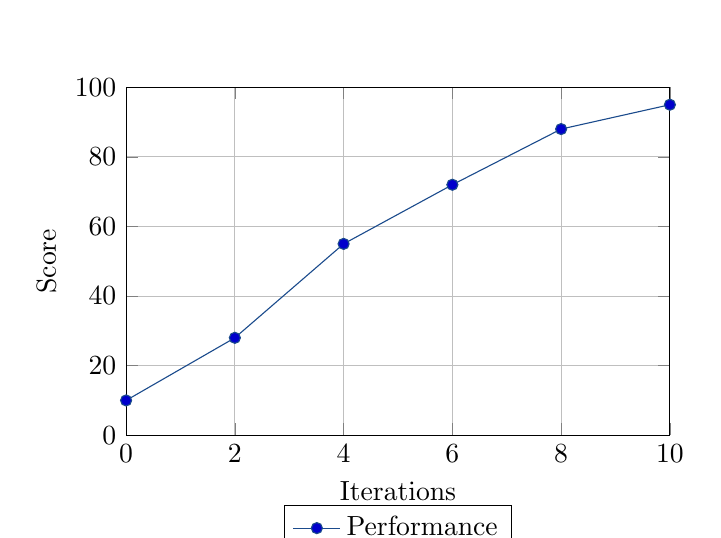
\begin{tikzpicture}
    \begin{axis}[
        width=0.7\textwidth,
        height=6cm,
        grid=both,
        xlabel={Iterations},
        ylabel={Score},
        xmin=0, xmax=10,
        ymin=0, ymax=100,
        legend style={at={(0.5,-0.2)},anchor=north}
      ]
      \addplot+[mark=*,color=fastprimary] coordinates {
        (0,10) (2,28) (4,55) (6,72) (8,88) (10,95)
      };
      \addlegendentry{Performance}
    \end{axis}
  \end{tikzpicture}
  \caption{PGFPlots example graph generated without external assets.}
  \label{fig:pgfplots-example}
\end{figure}

\section{Code Listings}

Source code is rendered using the \texttt{listings} package with the default style defined in \texttt{config/style.tex}. Adjust \texttt{\textbackslash TemplateCodeListingStyle} in \texttt{options.tex} to point to a different style.

\Cref{lst:js-running-total} demonstrates an inline listing embedded directly in the document for short examples. The more extensive Python and C++ modules now live in Appendix~\ref{app:code-samples}, keeping the main narrative focused while still providing full source listings for reference.

\begin{lstlisting}[style=githubJavaScript, caption={Running total helper implemented in modern JavaScript.}, label={lst:js-running-total}]
export function runningTotal(values) {
  let total = 0;
  return values.map((value) => {
    total += value;
    return total;
  });
}

console.log(runningTotal([4, 8, 15, 16, 23, 42]));
\end{lstlisting}

\section{Referencing}

Manage bibliography entries in \texttt{bib/references.bib}. The template uses \texttt{biblatex} with the \texttt{biber} backend for flexible citation styles.

\nocite{*} % Include all entries in the bibliography for the demo build.


% === References & Appendix ===
\newpage
\printbibliography

\clearpage
\appendix
\pagenumbering{Roman}
\section{Appendix Example}

Appendices are input after \texttt{\textbackslash appendix} is declared in \texttt{main.tex}. Use this space for supplementary derivations, raw data, or extended proofs that support the main text.

\subsection{Supplementary Code Listings}
\label{app:code-samples}

The full Python and C++ utilities referenced in \cref{lst:js-running-total} are provided here for completeness.

\lstinputlisting[
  style=githubPython,
  caption={Python helper for computing descriptive statistics.},
  label={lst:appendix-python}
]{assets/code/example.py}

\lstinputlisting[
  style=githubCpp,
  caption={C++ program computing the arithmetic mean of a sample.},
  label={lst:appendix-cpp}
]{assets/code/example.cpp}

\subsection{Just some text}
Lorem ipsum dolor sit amet, consectetur adipiscing elit. Sed do eiusmod tempor incididunt ut labore et dolore magna aliqua. Ut enim ad minim veniam, quis nostrud exercitation ullamco laboris nisi ut aliquip ex ea commodo consequat. Duis aute irure dolor in reprehenderit in voluptate velit esse cillum dolore eu fugiat nulla pariatur. Excepteur sint occaecat cupidatat non proident, sunt in culpa qui officia deserunt mollit anim id est laborum.

\end{document}
